 
 
\chapter{Applikasjon} 
 
 
I dette kapittelet vil det bli gjort rede for utviklingen og de applikasjonen. 
 
 
\section{Utgangspunkt} 
\label{sec:utgangspunkt} 
 
 
Målet med forskningen er å undersøke potensielle forbedringer funksjonene beskrevet i seksjon \ref{sec:ResearchQuestion} kan ha på den eksisterende løsningen Tobii Sono Flex (\ref{chap:Tobii-Sono-Flex}). Det mest naturlige valget for å implementere disse funksjonene ville vært å ta utgangspunkt i den eksisterende kildekode og utvidet med nødvendig kode. Problemet var at plattformen som den eksisterende koden var bygget på hadde flere begrensninger og ville gjort det vanskelig å fått implementert mye av funksjonalitet som skulle undersøkes, spesielt gjelder dette animasjonene. Dette gjorde at utviklingen ble startet som et nytt prosjekt og at første del av utviklingen var å lage en forenklet prototype av den samme applikasjonen bare på en annet rammeverk. 
 
 
\section{Kravspesifikasjon} 
 
 
Prototypen som skal bygges skal ikke ha all funksjonaliteten som Sono Flex har, men nok til at den greier å utføre hovedoppgaven. Som vil si at brukeren har mulighet til å skrive setninger med symboler for så å gjøre om disse til naturlig tale. For å kunne gjennomføre dette er det flere mindre oppgaver som må implementeres.  De ulike kravene vil bli beskrevet etter prioritert der de første er de mest nødvendige og kjent som kjernefunksjonalitet, deretter vil funksjonalitet som hadde vært greit å ha, men som ikke er nødvendig for applikasjonen skal kjøre.  
 
 
\subsection{Funksjonelle krav} 
 
 
 
 
Øyesporing som interaksjon - Det skal være mulig å kun bruke øyene til å operere prototypen. Det vil si at en som kun har mulighet til å bruke øyesporing skal kunne ta i bruk alle funksjonene som en har ved å bruke datamus.  Effektivitet skal væreså lik som mulig mellom de to interaksjonsformene. 
 
 
Logging - I systemet skal det være mulig å kunne logge all interaksjonen en bruker gjør med programvaren. Denne funksjonen vil være nødvendig for å kunne gjennomføre testingen 
 
 
Brukertilpasning - Hver bruker skal ha mulighet til å kunne tilpasse programvaren etter sine preferanser.  
  
Tale - Systemet skal kunne gjøre om teksten til ethvert symbol om til tale fra høyttalerne. Dette vil bli aktivert på brukerens kommando. Dette vil typisk være når en bruker har fullført en setning. 
  
Internasjonalisering - Systemet skal minimum ha språkstøtte for engelsk, norsk, svensk, tysk og dansk. 
 
 
Animasjon - I prototypen skal det være animasjoner som blir aktivert når en bruker trykker på de ulike symbolene.  
  
Lydeffekter - Utenom talelyden, skal det også være lydeffekter som skal avspilles ved brukerinteraksjon.  
 
 
Innlesning -  
 
 
Symbol - Hver brikke skal bestå av et ord og et symbol som representerer dette på best mulig måte. 
 
 
\subsection{Ikke-funksjonelle krav} 
 
 
Responstid -  Programvaren er kompleks og det tar lang tid å skrive med symboler, det er derfor viktig at systemet responderer kjapt og ikke gjør slik at oppgaven tar lenger tid. Slik at når brukeren trykker på noe skal det føles som om programvaren svarer momentant. 
 
 
Brukervennlighet - Målgruppen består av barn med som har begrenset erfaring med å operere dataprogrammer. Det er derfor viktig at det legges vekt på det og programvaren utformes på en måte som er intuitiv for brukeren.   
 
 
Fleksibilitet - Kodebasen skal være tilrettelagt for vedlikehold og videreutvikling. Det er viktig at personer som ikke har deltatt i systemutvikling enklest mulig skal kunne forstå koden og på den måten enkelt kan legge til og fikse funksjoner. Programvaren skal også legge oppp til at det er enkelt og legge til animasjoner, lyd og nye brikker. 
 
Personvern - Brukerne av programvaren er en sårbar gruppe, det vil derfor være vikitg at sensitiv informasjon om disse ikke kommer på avveie. Det skal i utgangspunktet ikke lagres sensitiv data, men det hvis data lagres skal det lagres på en sikker måte. 
 
 
 
 
\section{Utvikling} 
 
 
I denne seksjonen vil teknologier og arbeidsområde bli beskrevet, som skal gi grunnlag for den neste seksjonen som vil gå mer innpå implementasjon valg og detaljer. 
 
 
 
 
\subsection{Rammeverk} //Skriv mer om  grunnen til at det eksisterende rammeverket ikke var nok 
 
 
Siden grunnen til at utviklingen begynte med blanke ark var begrensninger i det eksisterende rammeverket, var det viktig at den nye som applikasjonen skulle bygges på, ikke hadde dem. Valget ble derfor basert på at den var tilrettelagt for implementering av ønsket funksjonalitet. Det vil si god støtte for brukergrensesnitteknologi som animasjon, lyd og bildebruk. En begrensing var at rammeverket måtte være kompatibelt med øyestyringsenheten Tobii PCEye GO. Dette gjorde at alternativene ikke var mange.  
Valget falt derfor på Microsoft .NET. Grunnen til dette var at rammeverket oppfylte alle kravene og er godt dokumentert. 
 
 
Arkitekturen til .NET er omfattende og som en kan se utfra figur \ref{fig:net-arkitektur} er det flere programmeringsspråk og komponenter en kan velge å ta i bruk. Rapporten vil derimot kun gi informasjon om de ulike komponentene fra .NET som ble brukt og er nødvendig for videre lesning. 
 
 
\begin{figure}[ht] 
\centering 
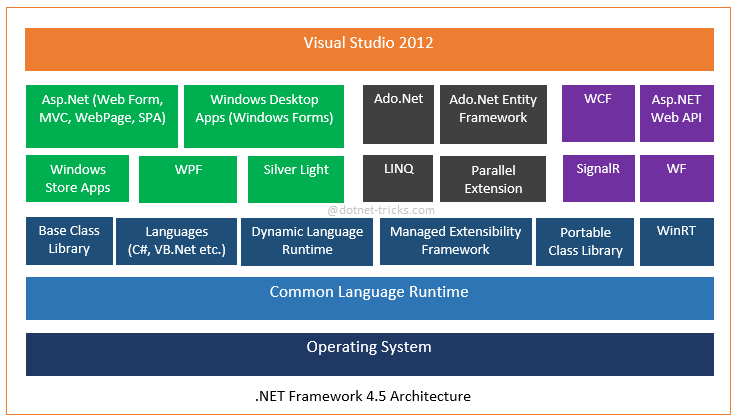
\includegraphics[width=140mm]{netframework45} 
\caption{Diagram som viser arkitekturen til .net rammeverket versjon 4.5} 
\label{fig:net-arkitektur} 
\end{figure} 
 
 
\subsection{Teknologi} 
 
 
Innenfor .NET sto valget mellom teknologiene Windows Store Apps, Windows Presentation Foundation(\gls{WPF}), Windows Forms og Silverlight.  Windows Forms ble utelukket ettersom dette er teknologien som Sono Flex er bygget på og som hadde begrensinger som gjorde at flere ønskede funksjoner ble vanskelig å implementere. Windows Store Apps hadde mye av den ønskede funksjonaliteten, samtidig som den fortsatt vedlikeholdes. For å distribuere slike applikasjoner brukes Windows Store. Problemet er at for å få publisert applikasjonen der, kreves godkjenning av Windows. En tidkrevende prosess, og med tanke på at applikasjonen antageligvis vil oppdateres hyppig kan dette bli et problem. Dette i sammenheng med at disse applikasjonene ikke er kompatible med Windows 7\cite{Windo0:online} gjorde at denne teknologien ble valgt bort. Til slutt sto valget mellom Silverlight og WPF. Silverlight er en kryssplattform, kryss web implementasjon av .NET rammeverket som har god støtte for grafiske elementer, animasjon og audio, og derfor en god kandidat. Funksjonaliteten i silverlight er et subset av WPF, som vil si at WPF minst har samme funksjonalitet som silverlight. Med unntak av Deep Zoom en funksjon som applikasjonen ikke hadde spesifikk behov for \cite{WPFvsSilverlight:online}. I tillegg til å tilby mer funksjonalitet var også bruk av wpf sammen med øyesporingsenheten beskrevet i enhetens dokumentasjon. Noe som vil gjøre prosessen med å integrere øyesporing i applikasjonen lettere. Dette gjorde at vi bestemte oss å utvikle i WFP. 
 
 
 
 
\section{Windows Presentation Foundation} 
 
 
Ifølge Adam Nathan \cite[p.~9]{WPFbook}, programvare arkitekt hos Microsoft er grunnen til at WPF ble lansert er at til tross for grafikk maskinvare hele tiden har blitt bedre og billigere og  forbrukerens forventninger fortsatt å stige, så er det ingen som har adressert vanskeligheten med å lage moderne brukergrensesnitt ref{Adam nathan bok side 9}.  Han argumenterer med at ja det fantes utviklere på tiden som for eksempel brukte bitmap bilder til å lage kulere knapper istedenfor å bruke standardknapp kontrollen. Problemet er at disse formene fort tilpasning ikke bare kan være ressurskrevende å utvikle, men også gi en dårligere brukeropplevelse. Nathan forteller derfor at Microsoft innså at det var et behov for noe helt nytt som ikke hadde de samme begrensningene som GDI+ og USER ga, men som samtidig hadde produktiviteten som folk likte fra rammeverk som Windows Forms. Sammen med at applikasjoner bygget med HTML og Javascript steg i popularitet. Trengte Windows en teknologi som var like morsom og enkel å bruke som disse, men samtidig som den utnyttet kraften den aldri-stoppende utviklingen av maskinvare har gitt. Resultatet ble Windows Presentation Foundation. 
 
 
   
\section{Arbeids område} 
 
 
For å automatisere mye av utviklingen ble det valgt å bruke utviklingsmiljøet Visual Studio 2013 \cite{2013-1:online}. Grunnen til at Visual Studio ble valgt er det for at i tillegg til å ha koderedigeringsverktøy og debugger, så har den også en WPF designer\cite{What8:online}. Denne designeren tilbyr flere hjelpemidler for å effektivisere prosessen med å lage brukergrensesnitt. Blant annet kan man velge mellom å kode de forskjellige elementene eller man kan dra dem inn fra et sidepanel. Den viktigste er derimot design vinduet, som til enhver tid viser hvordan brukergrensesnitt blir uten å måtte kjøre koden\cite{WPF D1:online}. 
 
 
For versjonskontroll ble det på grunn av erfaringsmessige årsaker brukt git\cite{AboutGit:online}. Til å ta backup av git filene ble den web-baserte tjenesten Bitbucket brukt. Grunnen til dette var mye av koden fra Tobii Dynavox var konfidensiell og Bitbucket tilbyr gratis hemmelig oppbevaring. 
 
 
 
 
 
 
 
 
 
 
 
 
\section{eXtensible Application Markup Language} 
 
 
 WPF bruker eXtensible Application Markup Language (\gls{XAML}), som er et XML-basert språk til å definere og kombinere ulike grensesnittelementer. Figur \ref{lst:myLabel} viser hvordan et vindu med en knapp er definert i XAML. Resultatet kan ses i figur \ref{fig:xamlButton}.  
 
 
\begin{lstlisting}[language=java,caption={Kodesnutt skrevet i XAML som viser en enkel applikasjon med en knapp} 
\label{lst:myLabel}, belowcaptionskip=4pt] 
<Window xmlns="http://schemas.microsoft.com/winfx/2006/xaml/presentation" Title="Window with Button"  Width="250" Height="100"> 
 
 
  <Button Name="button" Click="button_Click">Click Me!</Button> 
   
</Window> 
\end{lstlisting} 
 
 
\begin{figure}[ht!] 
\centering 
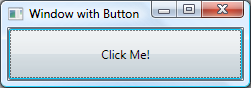
\includegraphics[width=100mm]{xamlButton} 
\caption{Skjermdump av det applikasjonen som blir gjengitt ved kjøring av kodefnutt \ref{lst:myLabel}} 
\label{fig:xamlButton} 
\end{figure} 
 
 
 
 
For å kunne samhandle med de grafiske objektene definert i XAML filen opprettes det alltid en tilhørende kodefil sammen med denne. Kodefilens formål er å ta seg av data og logikk for å ha et klart skille mellom utseende-spesifikk kode og oppførsel-spesifikk kode. For eksempel så vil en knapp sitt utseende og plassering bli definert XAML filen, mens hvordan data blir påvirket av interaksjon med knappen blir definert i den tilhørende kodefilen. 
 
 
Den tilhørende kode-filen til XAML koden beskrevet i kodesnutt \ref{lst:myLabel} er vist i kodesnutt \ref{lst:backbutton}. Ved å trykke på knappen bildet vil metoden button\textunderscore Click i kodefilen bli kalt og en dialogboks vist til brukeren. 
 
 
En XAML fil definerer som tidligere nevnt grafiske objekter som vindu, side eller brukerkontroll, men for at en bruker skal kunne samhandle med applikasjonen trengs de 
 
 
Vindu inneholder er en konteiner som inneholder alle applikasjonens grafiske elementer. En 
 
 
For å håndtere logikken og interaksjon med brukergrensesnittet,  definert i XAML, brukes det en kode fil. For hver XAML   Dette gjør at koden har et klart skille mellom utseende-spesifikk kode og oppførsel-spesifikk kode. 
 
 
Som tidligere nevnt defineres brukergrensesnittet i XAML, 
 
 
WPF oppfordrer til å skille mellom utseende spesifikk kode og oppførsel-spesifikk kode ved at grafiske elementer skrives i XAML og interaksjonen  kun brukes til generere  
XAML brukes til å generere brukergrensesnitt,  
Hver XAML-fil har en tilhørende kode-fil for håndtering av hendelser og oppførsel. Dette gjør at koden har et klart skille mellom utseende-spesifikk kode og oppførsel-spesifikk kode. Den tilhørende kode-filen til XAML koden beskrevet i kodesnutt \ref{lst:myLabel} er vist i kodesnutt \ref{lst:backbutton}. Ved å trykke på knappen bildet vil metoden button\textunderscore Click i kodefilen bli kalt og en dialogboks vist til brukeren. 
 
 
\begin{lstlisting}[language=java,caption={falafel} 
\label{lst:backbutton}] 
 void button_Click(object sender, RoutedEventArgs e) 
        { 
         Viser en dialogboks naar knappen trykkes 
        MessageBox.Show("Hallo!"); 
        } 
\end{lstlisting} 
 
 
\section{Model View ViewModel} 
 
 
En viktig del av oppgaven var å bygge en prototype som Tobii Dynavox kunne bygge og teste videre på. Det var derfor en forutsetning at kildekoden var tilrettelagt for vedlikehold og videreutvikling. For å gjennomføre dette valgte vi å følge arkitekt mønsteret Model view viewmodel (MVVM). Grunnen til at vi valgte nettopp dette foran andre mønster, som for eksempel Model View Contoller(MVC)\{MVC a2:online} eller Model-View-Presenter(MVP)/cite{The M4:online} er fordi WPF er designet for å lage applikasjoner med MVVM, Microsoft brukte selv MVVM til å utvikle WPF \cite{THEM6:online}. Det er mulig å bruke andre mønster, men det virket med dette argumentet mest logisk og velge MVVM. 
 
 
MVVM skal hjelpe utviklerne til med å separere forretnings- og presentasjonslogikk i applikasjonen fra brukergrensesnittet \cite{Im1online}. Ved å vedlikeholde er klar skille mellom applikasjons logikk og brukergrensesnitt skal det ifølge Microsoft \cite{Im1online}, gjøre det enklere å teste, vedlikeholde og videreutvikle.  
 
 
\begin{figure}[ht!] 
\centering 
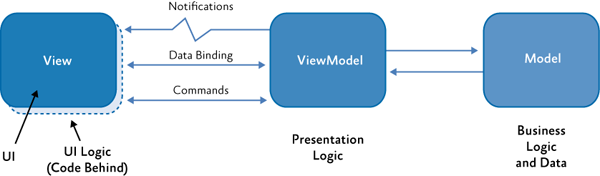
\includegraphics[width=100mm]{Mvvm} 
\caption{Illustrasjon som viser tre MVVM klasser og hvordan interaksjonen mellom dem\cite{Im1online}} 
\label{fig:mvvm} 
\end{figure} 
 
 
Figur \ref{fig:mvvm} viser de tre MVVM klassene view, view-model og model, og interaksjonen mellom disse. I view klassen defineres de visuelle elementene som vinduer, knapper, tekst, farger og organiseringen av dem. Med andre ord, selve brukergrensesnittet.  For at en bruker skal kunne utføre kommandoer og hente data gjennom et view, brukes det i WPF, databindings uttrykk som blir evaluert opp mot viewets gitte datakontekst. I MVVM vil datakonteksten være satt til viewmodellen. Det vil si som figur \ref{fig:mvvm} viser, at alle former for kommandoer, notfikasjoner og databinding skjer gjennom viewmodellen. Et view vil typisk kun forholde seg til en viewmodel, altså et en-til-en relasjon\cite{ite{THEM6:online}.   
 
 
Mens viewet bestemmer hvordan applikasjonen skal se ut, så bestemmer viewmodellen hvordan funksjonaliteten skal være \cite{THEM6:online}. Det er i viewmodellen at egenskaper og kommandoer som viewet kan binde seg opp mot er implementert. Når data  da endres vil view bli varslet og oppdatert deretter(Notified i figur \ref{fig:mvvm}) . På samme måte vil viewet kalle på viewmodellen om at en kommando må kjøres hvis for eksempel en bruker trykker på en knapp. Det er også Viewmodellen sitt ansvar og koordinere interaksjoner med viewet med de modellene som trengs. Det vil si at viewmodellen kan eksponere modellen direkte til viewets slik at de kan bindingen kan skje direkte til dem. Samtidig kan viewmodellen også manipulere data fra modellen , som for eksempel å kombinere to verdier. Eksempel kan være å sette sammen fornavn og etternavn fra en Person modell. Mens forholdet mellom View og Viewmodellen typisk er en-til-en, så vil ViewModellen ha en en-til-mange relasjon.  
 
 
\subsection{MVVM light} 
 
 
//Siden ny utvikling og lage en testplattform, viktig at kode var optimalisert 
//Mvvm passet best skille mellom logikk og blablabla 
//Vikitg å få med design time data, side applikasjonen er svært design tung 
//Finn fordeler 
//mvvm light  - IOC container, design data. 
//Arkitektur 
 
 
 
 
 
 
\section{Utvikling}  
 
 
I seksjon \ref{sec:utgangspunk} ble teknologien som ble brukt til å utvikle prototypen diskutert. I denne seksjonen vil arkitektturen og de viktigste utviklingsdetaljene  bli drøftet.  
 
 
\subsection{arkitektur} 
 
 
Figur \ref{fig:arkitektur} viser et forenklet bilde over hvordan klassene i kodebasen er koblet sammen. Med forenklet så menes det at flere hjelpeklasser og tredjeparts bilioteker er med i diagrammet. I tilegg så har ikke Views blitt tatt med i diagrammet, men for hver ViewModel så er det View som representerer det.  
 
 
 
 
\begin{figure}[ht] 
\centering 
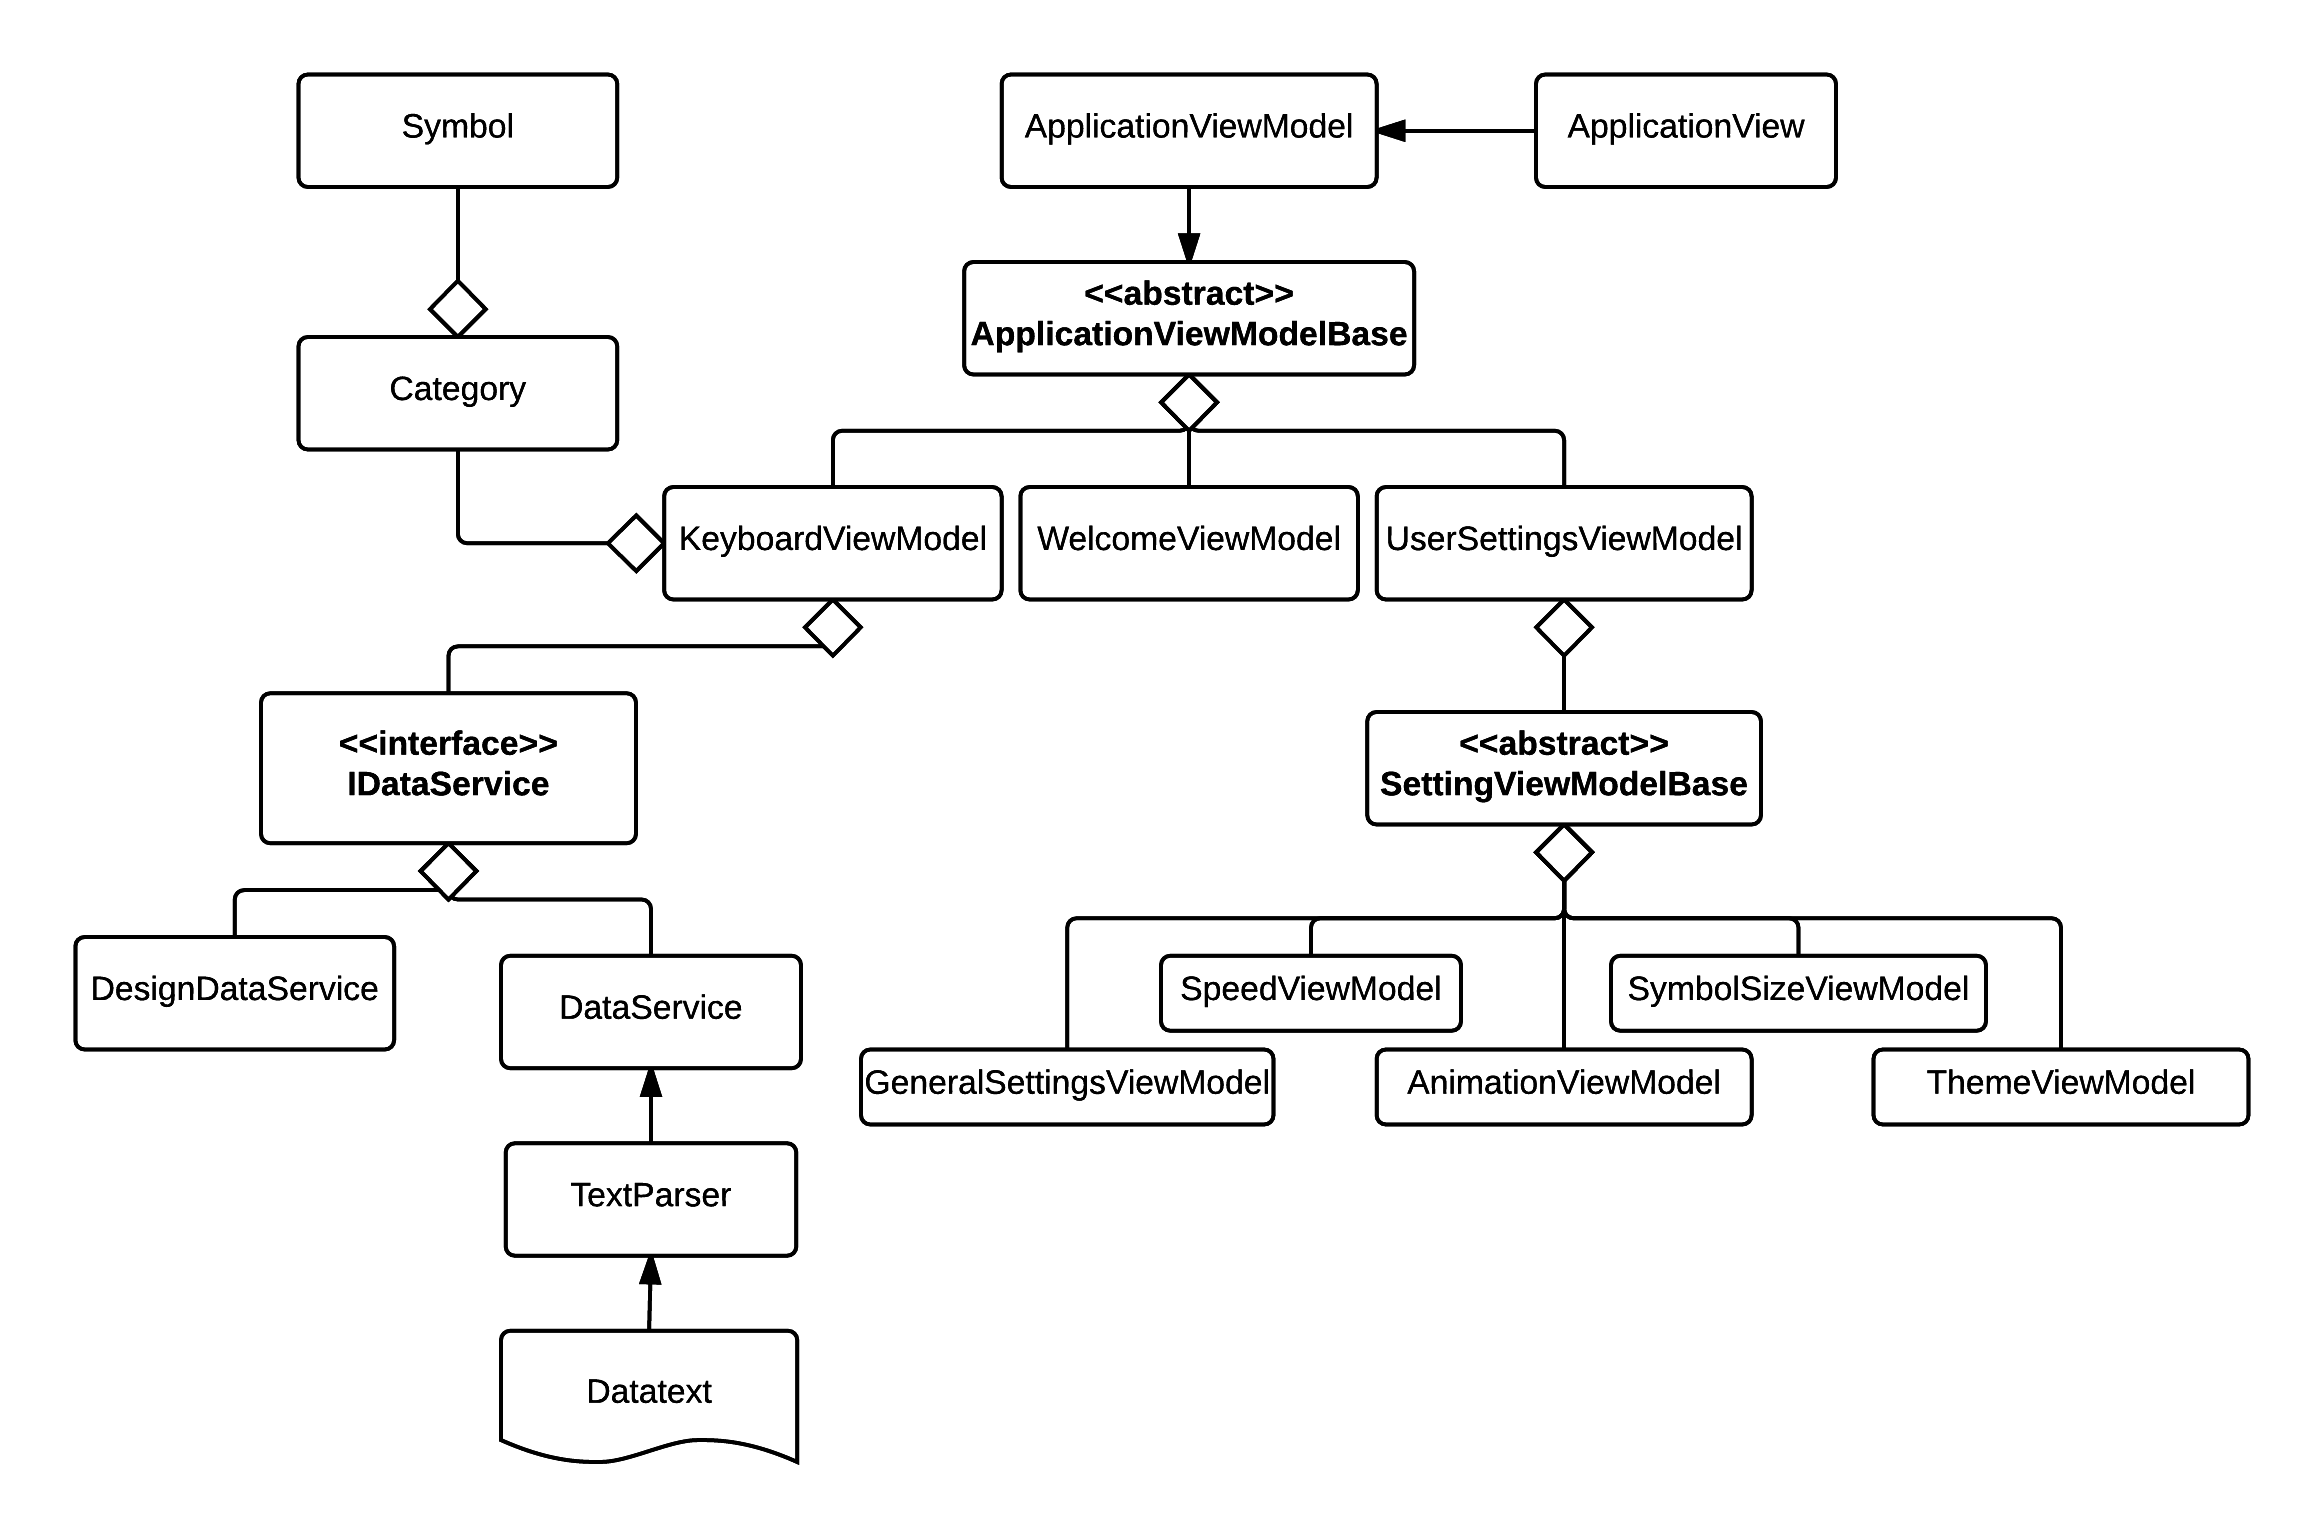
\includegraphics[width=140mm]{Arkitektur} 
\caption{Figur som viser et overordnet bilde av hvordan de ulike klassene henger sammen} 
\label{fig:arkitektur} 
\end{figure} 
 
 
 
 
 
 
 
 
 
 
ApplicationViewModel er vinduet som åpnes når programmet startes. Denne klassen fungerer som en kontainer for applikasjonen og bestemmer kun applikasjonsvinduets størrelse og navigasjon mellom de andre viewmodellene Keyboard, Welcome og UserSettings.  
 
 
\begin{listing}[ht] 
\inputminted{xml}{Code/ApplicationContainer.xml} 
\caption{Utdrag fra kode som viser hvordan kontainer er satt opp} 
\label{listing:Kontainer} 
\end{listing} 
 
 
\begin{listing}[ht] 
\inputminted{csharp}{Code/CurrentApplicationView.cs} 
\caption{Utdrag fra kode som viser hvordan kontainer er satt opp} 
\label{listing:CurrentAppView} 
\end{listing} 
 
 
 
 
Figur \ref{listing:Kontainer} viser hvordan ContentControl elementet i ApplicationView fungerer som en kontainer ved at innholdet er bundet til egenskapen CurrentViewModelBase. Som vil si at innholdet i ContentControl vil basere seg på hva som er satt som CurrentViewModelBase i ApplicationViewModel. Figur\ref{listing:CurrentAppView} viser hvordan denne egenskapen er implementert i Viewmodellen. Utfra koden så kan man se at til forskjell fra viewet, som hadde en referanse til egenskapen, så er det ingen direkte referanse fra viewmodellen til viewet. Dette er for å følge prinsippet til MVVM om at viewmodellen ikke skal ha noe kjennskap til Viewet, som gjør koden løs koblet(les: loose coupled). Men siden dette er en verdi som antakeligvis vil endre seg i løpet av kjøretiden er det nødvendig at Viewet blir gjort oppmerksom på forandring. Dette skjer ved å avfyre RaisePropertyChanged, dette kallet vil varsle rammeverket om at en endring har skjedd. Når da Viewet har en binding til denne egenskapen vil han bli oppmerksom på endringen og oppdatere deretter \cite{MVVM4:online}. 
 
 
CurrentViewModelBase er av typen ApplicationViewModelBase som vil si at det som er i kontaineren må være av nettopp denne typen. ApplicationViewModelBase er som man ser utifra figur  en abstrakt og har kun en abstrakt metode for å hente navn.  Det vil si at de klassene som arver fra ApplicationViewModel må implementere metoden. Fra figur kan man se at de klassene som arver fra ApplicationViewModel og med det har mulighet til å være i kontaineren er, KeyboardViewModel, UserSettingsViewModel og WelcomeViewModel. Sammen representerer disse hoved funksjonaliteten til programvaren. KeyboardViewModel er hoveddelen av applikasjonen, det her en bruker har mulighet til å skrive setninger med å trykke på de ulike symbolene for så å gjøre dem om til tale. I UserSettings kan en bruker se og endre på de ulike innstillingene. Mens WelcomeViewModel er kun laget for testingen og funksjonaliteten er begrenset til at en bruker kan velge alder og kalibrere øyesporingsenheten. 
 
 
 
 
 
 
 
 
 
 
 
 
 
 
 
 
 
 
 
 
 
 
 
 
 
 
 
 
\section{SymbolStix} 
 
 
En viktig del av programvaren er å hjelpe barn å bygge et vokabular ved å visualisere ord med bilder. Det vil si at for hvert ord må det finnes et bilde, noe som kan bli svært mange. Tobii Sono Flex har løst denne oppgaven med å bruke et kommersielt tredjeparts bildebibliotek kalt SymbolStix \cite{n2y}, utviklet av n2y. Bildene i biblioteket består av svært enkle tegninger som kun har med det mest nødvendige får å få frem konseptet eller ordet symbolet prøver å representere. Det at Sono Flex og at dette bildebiblioteket var tilgjengelig gjennom Tobii gjorde at den samme bildepakken skulle bli brukt i prototypen. Dette gjorde også medføre at ikke unødvendig med ressurser ble brukt på anskaffe bilder for hvert ord. 
 
 
 
 
\section{Problem} 
 
 
Symbolstix bildene er lagret i Enhanced Metafile Fomat (EMF), som er et 32-bit format som kan inneholde både vektor og bitmap informasjon\cite{AboutEMF}. Problemet med EMF formatet er at det ikke finnes støtte for dette i WPF, med den begrunnelse at det har blitt funnet en kritisk sårbarhet\cite{EMFVulnerability} og at formatet er mer mottakelig for sårbarheter\cite{EMFForum} enn andre bildeformater. I Sono Flex fungerer dette fint, fordi det bygget på Windows Forms(WF),  et rammeverk som har innlagt støtte for EMF. WPF har støtte for å bruke WF elementer,  en funksjon som ble lagt inn for å lette overgangen fra WF til WPF. Som igjen gjorde det mulig å hente bilder med EMF format. Ulempen er at man må trekke inn store deler av WF biblioteket noe som fører til en betraktelig økning i størrelse. For å aktivere støtten, deklarerer en WindowsFormHost i xaml filen og denne vil fungere som en kontainer for alle WF elementer. Innenfor denne kontaineren vil alt fungere som i et WF miljø. Ved å gjøre dette ble alle bildene hentes og vist i prototypen.  
 
 
Testing av applikasjonen viste derimot at det ikke lenger var mulig å trykke på knappene, eller mer korrekt, det var ikke mulig å trykke på  bildet der knappen var. Dette viste seg å være kjent problem, og er kjent som Airspace problemet (kilde) og kommer av at alle WF elementer uansett vil legge seg over alle WPF elementer. Et problem som ikke kunne være med i prototypen. En fix til dette ble laget og planlagt lansert i .NET versjon 4.5, men da versjonen ble lansert, var ikke denne fiksen med. Det finnes ulike omveier rundt på problemet, men få tilfredsstillende.  
 
 
Det ble derfor prøvd å konvertere EMF filene til bitmap for så å vise de i applikasjonen. Fordelen med denne fremgangsmåten var at vi slapp å trekke inn windows forms biblioteket. Ulempen var derimot at hver gang et symbol skulle hentes så måtte dette først konverteres til Bitmap for deretter og rendres. En tidkrevende prosess som gjorde at det tok flere sekunder å laste brukergrensesnittet. Det ble derfor prøvd å konvertere alle filene og deretter lagre dem som jpg. Konverteringen ville da kun gjøres en gang. Deretter ville applikasjonen hente jpg filene direkte, uten noe omvei. Siden wpf har innebygd støtte for formatet. Igjen viste det seg at dette ikke var godt nok ettersom jpg filene hadde blitt for store i overgangen fra vektor til raster grafikk og de manglet gjennomsiktighet. For mens EMF filene lå på under 10kb endte alle de konverterte filene opp på over 100kb. Noe som i selv ikke er så stort, men som gir utslag på lastingen av applikasjonen når det kan være opp mot 200 bilder som skal lastes. 
 
 
Den endelig løsningen ble å laste ned et profesjonelt konverteringsverktøy kalt AVS Image converter. En svært ømfintlig prosess som tok svært lang tid, men som gjorde det mulig å konvertere de orginale EMF filene til png og samtidig holde størrelsen på rundt 10 kb. 
 
 
 
 
 
 
 
 
 
 
\section{Layout} 
 
 
Prototypen har den samme layouten som Tobii Sono Flex, med en menylinje etterfulgt av en symboltabell under. Det er derimot en del variasjoner inne i hver av disse komponentene. 
 
 
\subsection{Menylinjen} 
 
 
Menylinjen dekker 1/5 del av applikasjonens vindu og består av 4 knapper og listen over ord som brukeren har trykket på. Denne listen vil heretter bli referert til som ordlisten. 
 
 
\subsubsection{Tilbaketasten} 
 
 
Tasten som befinner seg til høyre for ordlisten er tilbake tasten. Som på et vanlig tastatur vil et trykk på denne knappen medføre at det siste ordet i ordlisten fjernes. 
 
 
\subsubsection{Ordlisten} 
 
 
Når en bruker trykker på et ordsymbol så vil dette legge seg i ordlisten og når han trykker på "prate" knappen så vil ordene i listen bli gitt gjennom høyttalerne som naturlig tale og deretter fjernes fra listen. Selv om det er plass til uendelig med ord i listen så vil det kun være mulig for brukeren å se maks 4 om gangen.  Hvis det allerede er fire symboler i listen når brukeren trykker på et nytt symbol, så vil de tre første bli "fjernet" mens det fjerde og det nye symbolet vil være igjen. Hvis brukeren igjen fjerner de to siste ordene ved å trykke på tilbaketasten,  vil ordene som kommer før igjen bli presentert for brukeren.  
 
 
\subsubsection{Hjem} 
Ved å trykke på "hjem" knappen vil brukeren alltid bli ført til førstesiden av applikasjonen uavhengig av hvor han befinner seg.  
 
 
\subsubsection{Innstillinger} 
Hvis brukeren første er på "hjem" siden av applikasjonen så vil knappen byttes ut med en "innstillinger" knapp. Ved å trykke på denne vil det åpnes et nytt vindu hvor brukeren vil ha mulighet til å sette og endre på diverse innstillinger. Detaljene rundt denne siden er beskrevet i seksjon. 
 
 
\begin{figure}[ht!] 
\centering 
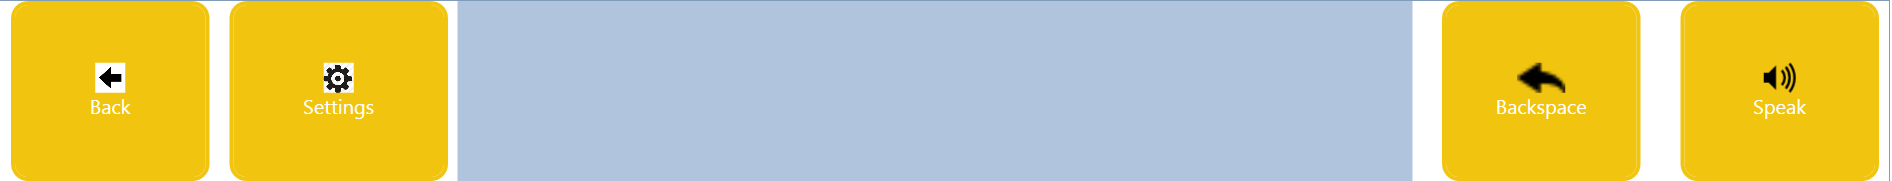
\includegraphics[width=100mm]{MenylinjeP} 
\caption{Skjermdump av menylinjen i prototypen \ref{lst:myLabel}} 
\label{fig:menylinjen} 
\end{figure} 
 
 
 
 
\section{Symboltabellen} 
 
 
Symboltabellen består av like mange kolonner og rader som den gjør i Sono Flex,  men det er måten den oppfører seg på som er annerledes.   
 
 
 
 
 
 
\section{Oppstart} 
hva skjer når applikasjonen startes. 
Leser fra fil 
Henter bilde2 
 
 
 
 
 
 
\section{Animasjon} 
 
 
Animasjoner i programvare brukes som et virkemiddel for å tiltrekke seg oppmerksomhet, underholde eller demonstrere noe. Det kan enten være en kort animasjon der en knapp tiltrer til en side når man svever over den med musen eller det kan være av den lengre sorten som en flash-video.  Animasjon er i hovedsak alt som beveger seg i applikasjonen. Selv om dynamikken som animasjoner kan fungere som et positivt virkemiddel viser undersøkelser gjort av Nielsen og Loranger \cite{NielsenBok}  at for mye blinkende og bevegende elementer kan slite ut brukeren og gjør det vanskeligere å fokusere på oppgaven. Med animasjonene som er implementer ønsker vi å undersøke dette. Hvilke animasjoner fungerer som et hjelpemiddel og med det gir verdi til applikasjonen og hvilke som er distraherende for brukeren og gir en uønsket effekt. 
 
 
I denne prototypen skjer animasjonene som en respons på at brukeren trykker på et symbol. Hva som skjer avhenger av hvilken type symbol det er. De ulike typene som finnes i symboltabellen ble forklart i seksjon \ref{subsubsec:symboltabell}, og er ordsymbol, kategorisymbol og navigasjonssymbol. 
 
 
 
 
\subsection{Animasjoner: ordsymbol} 
 
 
Når en bruker trykker på et ordsymbol, vil symbolet legge seg i setningslisten og er da klar for gjøres om til tydelig tale. Når brukeren har fullført setningen i Sono Flex blir brukeren presentert for endringen ved at symbolet vises i setningsfeltet. Med prototypen ønsker vi  å gi en mer visuell representasjon av denne endringen til brukeren. Ved å la brukeren kunne velge mellom to animasjoner som oppstår når han trykker på ønsket ordsymbol. De to animasjonene fungerer som følgende: 
 
 
 
 
I) Brukeren trykker på et ordsymbol. 
   Ordsymbolet krympes til 5 prosent av størrelsen. 
   I setningslisten vil en kopi av det krympede ordsymbolet dukke opp. 
   Kopien forstørres så til den opprinnelige størrelsen. 
   Ordsymbolet som opprinnelige ble trykket blir forstørret til opprinnelig størrelse. 
 
 
    
II) Brukeren trykker på et ordsymbol. 
    Ordsymbolet beveger seg ut av sin posisjon og glir mot den posisjonen den vil ha i setningslisten. 
    Når den har truffet posisjonen i setninglisten, stopper den opp og blir værende i ro. 
 
 
    Med disse animasjonen vil en først og fremst gi brukeren beskjed om at et valg har blitt gjort, men de ønsker også gjøre bruk av programvaren mer spennende.  I Sono Flex  vil ingen av knappene ha noe visuelt som gjør at brukeren kan skille hva som skjer, utenom at symboltabellen bytter ut de eksisterende symbolene. I dette tilfelle vil en se at symbolet går fra å være en statisk symbol til å bli flyttet til setningslisten og bli en del av ønsket setning.  
 
 
 
 
 
 
\subsection{Animasjon: Kategorisymbol} 
 
 
Når en bruker trykker på et kategorisymbol vil symbolene i symboltabellen byttes ut med symbolene som hører til i den gjeldene kategorien. Hvis en trykker på kategorien "dyr" så vil tabellen fylles med ordsymbol som "Hund", "katt", "tiger" o.s.v. Her ønsker animasjonen å hjelpe til med å fortelle at man ikke trykker på ordet dyr, men kategorien dyr og at brukeren får en forståelse for forskjellen mellom dem. Animasjonen startet ved at symbolet som brukeren trykket på forstørres helt til den dekker hele symboltabellen. Det vil si at ingen av de andre symbolene vises, kun kategorisymbolet. Symbolet vil så igjen forminskes, men symbolene i tabellen vil være erstattet av symbolene som tilhører kategorien.  
 
 
 
 
\subsection{Animasjon: Navigasjonssymbol} 
 
 
Den siste typen symbol er navigasjon og ved interaksjon vil den navigere mellom sider når det ikke er plass til alle symbolene på en side. Det vil si at symbolet skal kunne navigere fremover, fra side 1 til 2 og 2 til 3 og bakover igjen. Når brukeren trykker fremover starter animasjonen ved at alle symbolene som er på gjeldene side og neste side begynner å bevege seg mot venstre. Slik at symbolene på gjeldene side kontinuerlig blir byttet ut med de på neste. Symbolene på siden sklir ut, mens symbolene på neste sklir inn og overtar plassene. Når brukeren nå trykker på bakover-symbolet vil det samme skje bare at symbolene sklir mot høyre. 
 
 
\section{Lydeffekter} 
 
 
Som en del av rapporten ønsket vi å undersøke hvilken påvirkning lydeffekter hadde på brukeren. Hovedsakelig var målet å finne ut to ting. I hvilken grad hjelper effektene brukeren i å navigere rundt i applikasjonen og om det vil påvirke brukerens helhets uttrykk av applikasjonen.  
 
 
\subsection{Lydeffekter i prototypen} 
 
 
I prototypen er det lagt til flere lydeffekter, utelukkende i form av små lydklipp på maks 1 sekund. Effektene vil kun bli avspilt som en respons til noe brukeren foretar seg eller som å informere om en hendelse. Denne begrensning finnes for å ikke skape forvirring hos brukeren. Hvis lyd også hadde blitt avspilt tilfeldig så ville meningen med effektene forsvinne. Fordi brukeren blir lurt til å tro at programvaren har registrert en interaksjon, selv om han ikke har foretatt seg noe. Det er derfor viktig at det er lett for brukeren å skille mellom effektene som representerer en interaksjon og informasjon. De ulike interaksjonslydeffektene er også forskjellige, og hvilken som blir spilt er avhengig av,  som med animasjon,  hvilken type komponent brukeren samhandler med. Eksempelvis vil lyden som blir avspilt når brukeren trykker å tilbaketasten representere noe som forsvinner.  
 
 
 
 
\begin{itemize} 
\item Symbolord - Enkel klikkelyd 
\item Kategoriord - usikker 
\item navigasjonsord - svisj 
\item Innstillinger - Verktøyskasse 
\item tilbaketasten/slett - forvsinner 
\item hjem - usikker 
\item prat 
\end{itemize} 
 
 
 
 
 
 
 
 
 
 
Dette vil forhåpentligvis gjøre at brukeren mer effektivt kan bekrefte valget og fortsette med oppgaven. Som  
 
 
 
 
 
 
 
 
Hvilken brukeren blir presentert for er avhengig av hvilket komponent han interagerer med.  Grunnen er at hvis effektene hadde blit avspilt uten at brukeren foretar seg noe, så kan 
 
 
 
 
Hvilken lyd som blir avspilt er avhengig av hvilket valg brukeren har foretatt seg, og responsen til brukeren vil  
 
 
Eksmepelvis hvis brukeren foretar seg et ulovlig valg vil han bli presentert for en lyd som har gir negative assosiasjoner.  D 
 
 
Lyden som vil bli gitt til brukeren vil komme i form av små lydklipp som maks vil vare i et sekund,  ettersom det skal være nok for at brukeren kan registrere det.  
 
 
 Tilbakemelding i form av lyd gir brukeren en bekreftelse på at han valget han nettopp har foretatt har blitt registrert og  
 
 
 
 
 
 
Ta for eksempel brødristeren. Når den er ferdig vil brødet hoppe opp, men i tilegg vil den gi fra seg et pling. Altså brukeren vil få tilbakemelding på at han kan hente brødet både visuelt(brødet som hopper opp) og gjennom lyd(plinget). Ved å g 
 
 
Lyd brukes ofte for å fortelle brukeren av produktet noe. For eksempel vil brødristen gi fra seg et pling når den er ferdig samtidig med at skivene hopper opp av maskinen. I dette tilfellet vil  
 
 
 
 
I dag brukes lyd ofte i flere sammenhenger, i alt fra 
 
 
 
 
 
 
\section{Sammendrag} 
 